% FILE: chapters/ch01_s5_visualization.tex
\section{Visualization}\label{sec:visualization}

In the preceding sections, we learned how to store numerical arrays with NumPy and manipulate tabular sensor datasets with pandas. However, inspecting raw arrays of numbers—even with summary statistics like mean and variance—can dangerously mislead an engineer.

Consider the famous mathematical demonstration known as \textbf{Anscombe's Quartet}: four distinct datasets that share the exact same mean ($9.0$), identical sample variance ($11.0$), the same correlation coefficient ($0.816$), and the identical linear regression line ($y = 3.00 + 0.500x$). Yet, when plotted visually, one dataset is linear, the second is a curved parabola, the third is a straight line with an extreme outlier, and the fourth is a vertical cluster of points dominated by a single leverage point. If you only look at summary statistics, you are flying blind.

In machine learning and IoT, data visualization is essential at two distinct phases:
\begin{enumerate}
    \item \textbf{Exploratory Data Analysis (EDA)}: Visualizing sensor distributions, detecting non-linear correlations, identifying clustering behaviors, and spotting physical sensor dropouts before modeling.
    \item \textbf{Model Diagnostics and Evaluation}: Plotting training loss curves to diagnose overfitting, visualizing confusion matrices to understand failure modes, and inspecting ROC curves to select optimal classification thresholds.
\end{enumerate}

In this section, we master Python's two premier visualization libraries: **Matplotlib** (the low-level rendering engine) and **Seaborn** (the high-level statistical interface).

\begin{figure}[htbp]
\centering
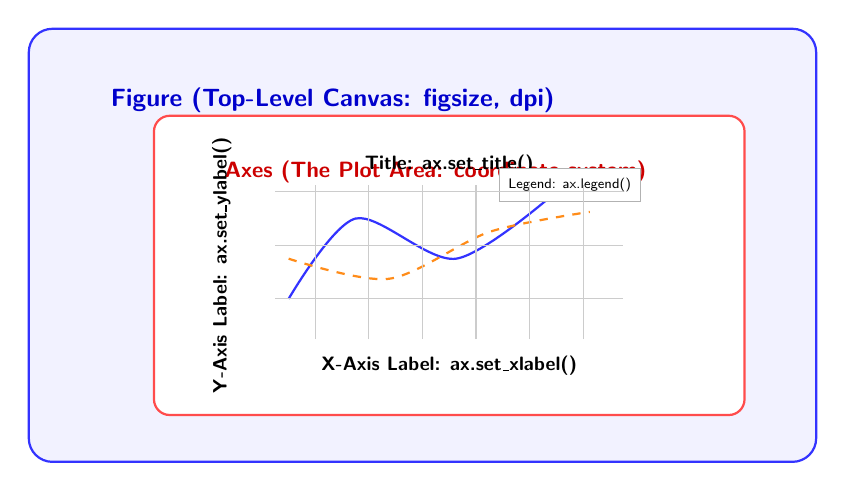
\begin{tikzpicture}[
    scale=0.85,
    figbox/.style={rectangle, draw=blue!80, fill=blue!5, rounded corners=3mm, thick, minimum width=10cm, minimum height=5.5cm},
    axbox/.style={rectangle, draw=red!70, fill=white, rounded corners=2mm, thick, minimum width=7.5cm, minimum height=3.8cm},
    element/.style={font=\scriptsize\sffamily\bfseries}
]
    % Figure Container
    \node[figbox] (fig) at (0, 0) {};
    \node[anchor=north west, font=\small\sffamily\bfseries, text=blue!80!black] at (-4.8, 2.5) {Figure (Top-Level Canvas: figsize, dpi)};

    % Axes Container
    \node[axbox] (ax) at (0.4, -0.3) {};
    \node[anchor=north west, font=\footnotesize\sffamily\bfseries, text=red!80!black] at (-3.1, 1.4) {Axes (The Plot Area: coordinate system)};

    % Plot Title & Labels
    \node[element, text=black] at (0.4, 1.2) {Title: ax.set\_title()};
    \node[element, text=black, rotate=90] at (-3.0, -0.3) {Y-Axis Label: ax.set\_ylabel()};
    \node[element, text=black] at (0.4, -1.8) {X-Axis Label: ax.set\_xlabel()};

    % Plot Data Elements
    \draw[thick, blue!80] plot[smooth] coordinates {(-2.0, -0.8) (-1.0, 0.4) (0.5, -0.2) (2.0, 0.8)};
    \draw[thick, orange!90, dashed] plot[smooth] coordinates {(-2.0, -0.2) (-0.5, -0.5) (1.0, 0.2) (2.5, 0.5)};

    % Annotations
    \node[rectangle, draw=gray!60, fill=white, font=\tiny\sffamily] at (2.2, 0.9) {Legend: ax.legend()};
    \draw[gray!40, step=0.8cm] (-2.2, -1.4) grid (3.0, 0.9);
\end{tikzpicture}
\caption{The hierarchical anatomy of a Matplotlib visualization: the Figure canvas containing one or more Axes plots.}\label{fig:matplotlib_anatomy}
\end{figure}

% ==============================================================================
% 1. MATPLOTLIB BASICS
% ==============================================================================
\subsection{Matplotlib: The Engine Room of Python Plotting}

\begin{keyidea}[Figure vs. Axes: The Object-Oriented Pattern]
Every Matplotlib visualization is governed by a strict two-tier object hierarchy:
\begin{itemize}
    \item \textbf{\code{Figure}}: The top-level bounding canvas or page upon which graphics are rendered.
    \item \textbf{\code{Axes}}: The actual coordinate plot box (with an x-axis, y-axis, title, and data lines) drawn inside the Figure. A single Figure can contain multiple sub-Axes (e.g., a $2 \times 2$ grid of plots).
\end{itemize}
Always use the **Object-Oriented (OO) API** (\code{fig, ax = plt.subplots()}) rather than the global state-machine interface (\code{plt.plot()}) to maintain precise control over complex subplots.
\end{keyidea}

\begin{analogy}[The Artist's Wooden Easel and Canvases]
Think of the \code{Figure} as a large wooden artist's easel set up in a studio. The \code{Axes} are the individual rectangular paper canvases you clip onto that easel. You can clip a single large canvas in the center, or you can clip four smaller canvases side-by-side to display four different views of the same subject.
\end{analogy}

\paragraph{Professional Subplot Architecture}
The following script demonstrates the standard, reproducible structure for creating multi-panel figures:

\begin{lstlisting}[language=Python]
import matplotlib.pyplot as plt
import numpy as np

# 1. Generate synthetic sensor telemetry
time_sec = np.linspace(0.0, 10.0, 500)
accel_vibration = 0.5 * np.sin(2 * np.pi * 1.5 * time_sec) + np.random.normal(0, 0.05, 500)
temp_celsius = 25.0 + 0.8 * time_sec + np.random.normal(0, 0.2, 500)

# 2. Instantiate a Figure with 2 vertically stacked subplots (2 rows, 1 col)
fig, (ax1, ax2) = plt.subplots(nrows=2, ncols=1, figsize=(8, 6), sharex=True)

# 3. Panel 1: Accelerometer waveform
ax1.plot(time_sec, accel_vibration, color='tab:blue', linewidth=1.2, label="Vibration (g)")
ax1.set_title("Machine Spindle Telemetry Stream", fontsize=12, fontweight='bold')
ax1.set_ylabel("Acceleration (g)")
ax1.grid(True, linestyle='--', alpha=0.6)
ax1.legend(loc="upper right")

# 4. Panel 2: Spindle temperature buildup
ax2.plot(time_sec, temp_celsius, color='tab:red', linewidth=1.5, label="Casing Temp ($^\circ$C)")
ax2.set_xlabel("Time Elapsed (seconds)")
ax2.set_ylabel("Temperature ($^\circ$C)")
ax2.grid(True, linestyle='--', alpha=0.6)
ax2.legend(loc="lower right")

# 5. Clean layout spacing and save publication-quality vector graphic
plt.tight_layout()
plt.savefig("sensor_telemetry.png", dpi=300, bbox_inches='tight')
plt.show()
\end{lstlisting}

\paragraph{Why \code{plt.tight_layout()} and \code{dpi=300} Matter}
\begin{itemize}
    \item \code{plt.tight_layout()}: Automatically adjusts subplot margins so axis numbers, titles, and labels do not overlap.
    \item \code{dpi=300}: Sets resolution to 300 Dots Per Inch, ensuring plots remain crisp in printed textbooks and reports without pixelation.
\end{itemize}

% ==============================================================================
% 2. SEABORN STATISTICAL PLOTS
% ==============================================================================
\subsection{Seaborn: Statistical Visualizations for Machine Learning}

\begin{keyidea}[Why Seaborn?]
**Seaborn** is a statistical data visualization library built directly on top of Matplotlib. While Matplotlib requires you to write low-level code to format ticks and legend entries, Seaborn operates directly on pandas DataFrames, automatically grouping categories, computing confidence intervals, and applying modern color palettes with a single line of code.
\end{keyidea}

To illustrate exploratory data analysis, we generate a synthetic factory sensor dataset with 1,000 samples:

\begin{lstlisting}[language=Python]
import pandas as pd
import seaborn as sns

# Configure consistent aesthetic theme
sns.set_theme(style="whitegrid", font_scale=1.0)

np.random.seed(42)
n_samples = 1000

# Synthetic dataset: Normal operation vs. Bearing Fault
is_fault = np.random.choice([0, 1], size=n_samples, p=[0.85, 0.15])
vibration_rms = np.where(is_fault == 1, 
                         np.random.normal(3.8, 0.6, n_samples), 
                         np.random.normal(1.2, 0.3, n_samples))
operating_temp = np.where(is_fault == 1, 
                          np.random.normal(68.0, 5.0, n_samples), 
                          np.random.normal(45.0, 3.5, n_samples))

df_sensors = pd.DataFrame({
    'vibration_rms_g': vibration_rms,
    'operating_temp_c': operating_temp,
    'machine_state': np.where(is_fault == 1, 'Bearing_Fault', 'Normal')
})
\end{lstlisting}

% ==============================================================================
% 3. FOUR CORE EXPLORATORY PLOTS
% ==============================================================================
\subsection{The Four Core Exploratory Plots}

\paragraph{1. Histograms and Kernel Density Estimation (KDE)}
A \textbf{Histogram} groups continuous measurements into discrete bins to show the empirical frequency distribution. A \textbf{Kernel Density Estimation (KDE)} smooths this histogram with a continuous probability density curve:
\begin{equation}
\hat{f}(x) = \frac{1}{n h} \sum_{i=1}^n K\left(\frac{x - x_i}{h}\right)\label{eq:kde}
\end{equation}
where $K(\cdot)$ is a Gaussian kernel and $h$ is the smoothing bandwidth.

\begin{lstlisting}[language=Python]
fig, ax = plt.subplots(figsize=(7, 4))
sns.histplot(
    data=df_sensors, 
    x='vibration_rms_g', 
    hue='machine_state', 
    kde=True, 
    palette={'Normal': 'tab:blue', 'Bearing_Fault': 'tab:red'},
    ax=ax
)
ax.set_title("Vibration Distribution: Normal vs. Faulty Machinery")
ax.set_xlabel("Vibration RMS (g)")
plt.show()
\end{lstlisting}
The resulting bimodal distribution immediately reveals that normal equipment vibrates below $2.0\text{ g}$, whereas faulty bearings produce a distinct Gaussian hump centered at $3.8\text{ g}$.

\paragraph{2. Scatter Plots with Categorical Hue}
Scatter plots reveal non-linear dependencies and cluster separability across two continuous features:

\begin{lstlisting}[language=Python]
fig, ax = plt.subplots(figsize=(7, 5))
sns.scatterplot(
    data=df_sensors, 
    x='operating_temp_c', 
    y='vibration_rms_g', 
    hue='machine_state',
    style='machine_state',
    alpha=0.7,
    palette={'Normal': 'tab:blue', 'Bearing_Fault': 'tab:red'},
    ax=ax
)
ax.set_title("Operational Phase Space: Temperature vs. Vibration")
ax.set_xlabel("Operating Temperature ($^\circ$C)")
ax.set_ylabel("Vibration RMS (g)")
plt.show()
\end{lstlisting}
If the two colored clusters form clean, non-overlapping islands, a linear classifier (such as Logistic Regression) will achieve high accuracy. If the clusters heavily interpenetrate, a non-linear classifier (such as a Random Forest or Neural Network) is required.

\paragraph{3. Box Plots and Interquartile Range (IQR) Outlier Fences}
A \textbf{Box Plot} summarizes a distribution through five key numbers: Minimum, First Quartile ($Q_1$), Median, Third Quartile ($Q_3$), and Maximum.

\begin{figure}[htbp]
\centering
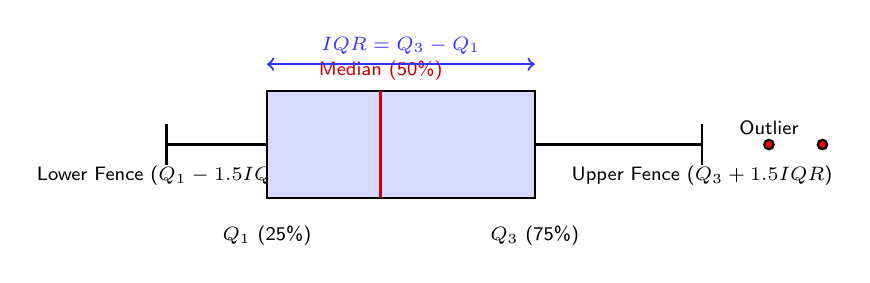
\begin{tikzpicture}[
    scale=0.85,
    thick
]
    % Lower Whisker
    \draw (0, 0) -- (1.5, 0);
    \draw (0, -0.3) -- (0, 0.3) node[below=4mm, font=\scriptsize\sffamily] {Lower Fence ($Q_1 - 1.5\text{IQR}$)};

    % Box
    \draw[fill=blue!15] (1.5, -0.8) rectangle (5.5, 0.8);
    \node[below=9mm, font=\scriptsize\sffamily] at (1.5, 0) {$Q_1$ (25\%)};
    \node[below=9mm, font=\scriptsize\sffamily] at (5.5, 0) {$Q_3$ (75\%)};

    % Median Line
    \draw[very thick, red!80!black] (3.2, -0.8) -- (3.2, 0.8) node[above, font=\scriptsize\sffamily] {Median (50\%)};

    % Upper Whisker
    \draw (5.5, 0) -- (8.0, 0);
    \draw (8.0, -0.3) -- (8.0, 0.3) node[below=4mm, font=\scriptsize\sffamily] {Upper Fence ($Q_3 + 1.5\text{IQR}$)};

    % Outliers
    \draw[fill=red] (9.0, 0) circle (2pt) node[above, font=\scriptsize\sffamily] {Outlier};
    \draw[fill=red] (9.8, 0) circle (2pt);

    % IQR annotation
    \draw[<->, blue!80] (1.5, 1.2) -- (5.5, 1.2) node[midway, above, font=\scriptsize\sffamily] {$\text{IQR} = Q_3 - Q_1$};
\end{tikzpicture}
\caption{Anatomy of a Box Plot: The Interquartile Range (IQR) and Tukey outlier fences.}\label{fig:boxplot_anatomy}
\end{figure}

The \textbf{Interquartile Range (IQR)} spans the middle $50\%$ of observations:
\begin{equation}
\text{IQR} = Q_3 - Q_1\label{eq:iqr}
\end{equation}
Data points extending beyond the whiskers are mathematically flagged as statistical outliers:
\begin{align*}
\text{Lower Outlier Fence} &= Q_1 - 1.5 \times \text{IQR} \\
\text{Upper Outlier Fence} &= Q_3 + 1.5 \times \text{IQR}
\end{align*}

\begin{lstlisting}[language=Python]
fig, ax = plt.subplots(figsize=(6, 4))
sns.boxplot(
    data=df_sensors, 
    x='machine_state', 
    y='operating_temp_c', 
    palette='Set2', 
    ax=ax
)
ax.set_title("Temperature Variance and Outliers Across States")
plt.show()
\end{lstlisting}

\paragraph{4. Correlation Heatmaps}
To inspect pairwise linear relationships across multiple physical sensor channels:
\begin{equation}
r_{xy} = \frac{\sum (x_i - \bar{x})(y_i - \bar{y})}{\sqrt{\sum (x_i - \bar{x})^2 \sum (y_i - \bar{y})^2}}\label{eq:pearson}
\end{equation}

\begin{lstlisting}[language=Python]
# Compute Pearson correlation matrix
corr_matrix = df_sensors[['vibration_rms_g', 'operating_temp_c']].corr()

fig, ax = plt.subplots(figsize=(5, 4))
sns.heatmap(
    corr_matrix, 
    annot=True,          # Display numeric r values in each cell
    fmt=".2f",           # Two decimal places
    cmap="coolwarm",     # Blue (-1) to Red (+1) divergent palette
    vmin=-1.0, vmax=1.0,
    square=True,
    ax=ax
)
ax.set_title("Sensor Feature Correlation Matrix")
plt.show()
\end{lstlisting}

% ==============================================================================
% 4. PLOTTING MODEL RESULTS
% ==============================================================================
\subsection{Plotting Machine Learning Diagnostics: Loss Curves and Confusion Matrices}

Once a model is trained, visualization provides the diagnostic tools needed to evaluate its learning dynamics and classification trade-offs.

\paragraph{1. Diagnosing Training Dynamics with Loss Curves}
A \textbf{Loss Curve} plots the loss function value on both the training set and validation set across training epochs. Comparing the two curves reveals the model's bias-variance state:

\begin{lstlisting}[language=Python]
# Simulated training and validation loss trajectories across 20 epochs
epochs = np.arange(1, 21)
train_loss = 0.8 * np.exp(-0.25 * epochs) + 0.05
val_loss = 0.85 * np.exp(-0.22 * epochs) + 0.10 + 0.003 * (epochs - 10)**2 * (epochs > 10)

fig, ax = plt.subplots(figsize=(7, 4))
ax.plot(epochs, train_loss, 'o-', color='tab:blue', linewidth=1.5, label='Training Loss')
ax.plot(epochs, val_loss, 's--', color='tab:orange', linewidth=1.5, label='Validation Loss')

# Annotate the optimal early stopping checkpoint
optimal_epoch = np.argmin(val_loss) + 1
ax.axvline(x=optimal_epoch, color='tab:green', linestyle=':', label=f'Optimal Checkpoint (Epoch {optimal_epoch})')

ax.set_title("Neural Network Learning Curves: Diagnosing Overfitting")
ax.set_xlabel("Epochs")
ax.set_ylabel("Cross-Entropy Loss")
ax.set_xticks(epochs)
ax.grid(True, linestyle='--', alpha=0.5)
ax.legend()
plt.show()
\end{lstlisting}

\begin{keyidea}[Visual Diagnosis from Loss Curves]
\begin{itemize}
    \item \textbf{Underfitting (High Bias)}: Both training loss and validation loss remain high and refuse to decrease. The model is too simple to capture the underlying pattern.
    \item \textbf{Optimal Generalization}: Both curves descend smoothly together and plateau.
    \item \textbf{Overfitting (High Variance)}: Training loss continues to decrease toward zero, but validation loss begins curving upward (diverging). The model is memorizing noise in the training set and losing the ability to generalize to new data.
\end{itemize}
\end{keyidea}

\paragraph{2. Normalized Confusion Matrix Heatmap}
While raw numbers in a confusion matrix can be hard to read, a normalized heatmap immediately highlights where the classifier makes systematic classification errors:

\begin{lstlisting}[language=Python]
from sklearn.metrics import confusion_matrix

# Simulated true and predicted labels on an edge test set
y_true = np.array([0]*900 + [1]*100)
y_pred = np.array([0]*880 + [1]*20 + [0]*15 + [1]*85)

# Compute normalized confusion matrix (fractions of true class)
cm = confusion_matrix(y_true, y_pred, normalize='true')

fig, ax = plt.subplots(figsize=(5, 4))
sns.heatmap(
    cm, 
    annot=True, 
    fmt=".1%",         # Display as percentages (e.g., 97.8%)
    cmap="Blues", 
    xticklabels=['Normal', 'Fault'],
    yticklabels=['Normal', 'Fault'],
    cbar=False,
    ax=ax
)
ax.set_title("Normalized Confusion Matrix")
ax.set_xlabel("Predicted Class")
ax.set_ylabel("Actual Ground Truth")
plt.show()
\end{lstlisting}

\begin{iotbox}[Visualizing Vibration Spectrograms for TinyML]
In predictive maintenance on microcontrollers, analyzing raw time-domain waveforms is often insufficient. High-frequency bearing defects produce distinct harmonics visible only in the frequency domain.

Using Matplotlib's \code{ax.specgram()}, an engineer can visualize a \textbf{Spectrogram}: a 2D heat map showing how frequency content evolves over time. A healthy motor shows steady low frequencies ($< 60\text{ Hz}$); an imminent bearing fault creates bright spectral lines at ultrasonic frequencies ($> 2{,}000\text{ Hz}$). This visual transformation guides whether an edge feature pipeline should extract FFT bins before passing data to an on-device classifier.
\end{iotbox}

\begin{warning}[Common Visualization Pitfalls]
\begin{itemize}
    \item \textbf{Overplotting}: When plotting 100,000 sensor points, points overlap into an unreadable solid blob. Always add transparency (\code{alpha=0.1}) or use density plots (\code{sns.kdeplot} or \code{ax.hexbin}).
    \item \textbf{Trunkated Axes}: Forcing a bar chart y-axis to start at $95\%$ to make a $1\%$ improvement look like a $500\%$ gain is misleading. Start zero-based charts at zero unless examining residuals.
    \item \textbf{Unlabeled Units}: Never label an axis simply as ``Temperature'' or ``Speed''. Always include physical units: \code{Temperature ($^\circ$C)} or \code{Speed (RPM)}.
\end{itemize}
\end{warning}

\begin{takeaways}
\begin{itemize}
    \item Never rely solely on summary statistics; visual inspection reveals non-linear patterns, clusters, and outliers.
    \item In Matplotlib, always use the Object-Oriented interface (\code{fig, ax = plt.subplots()}) for robust control.
    \item Use Seaborn for high-level statistical plotting (\code{histplot}, \code{scatterplot}, \code{boxplot}, \code{heatmap}).
    \item Box plots use the Interquartile Range ($\text{IQR} = Q_3 - Q_1$) to mathematically identify outliers beyond $1.5 \times \text{IQR}$.
    \item Loss curves visually expose underfitting, optimal generalization, and the onset of overfitting where validation loss diverges.
\end{itemize}
\end{takeaways}

% ==============================================================================
% 5. CHECK YOURSELF
% ==============================================================================
\subsection{Check Yourself}

\begin{enumerate}
    \item \textbf{Matplotlib Hierarchy}: What is the precise operational difference between a Matplotlib \code{Figure} and a Matplotlib \code{Axes}? Which object contains the title and axis labels?

    \item \textbf{Interquartile Range Outlier Calculation}: A vibration sensor records the following sorted readings in $g$:
    \begin{equation*}
    [0.10, \quad 0.20, \quad 0.25, \quad 0.30, \quad 0.40, \quad 0.50, \quad 0.90]
    \end{equation*}
    Given that the first quartile is $Q_1 = 0.20$ and the third quartile is $Q_3 = 0.50$:
    \begin{enumerate}[label=(\alph*)]
        \item Calculate the Interquartile Range ($\text{IQR}$).
        \item Calculate the Upper Outlier Fence ($Q_3 + 1.5 \times \text{IQR}$).
        \item Is the reading $0.90\text{ g}$ mathematically an outlier?
    \end{enumerate}

    \item \textbf{Diagnosing Overfitting}: You inspect a loss curve. At Epoch 5, training loss is $0.40$ and validation loss is $0.42$. At Epoch 25, training loss has dropped to $0.08$, but validation loss has climbed to $0.65$. What is the model experiencing? What corrective action should you take?

    \item \textbf{Overplotting in Sensor Telemetry}: You generate a scatter plot of $200{,}000$ accelerometer readings using \code{ax.scatter(x, y)}. The plot is a solid, opaque mass of black pixels. What two parameters or plot types should you use to make the density visible?

    \item \textbf{Confusion Matrix Heatmap Interpretation}: In a normalized confusion matrix heatmap, what does a strong dark square on the off-diagonal cell $(1, 0)$ indicate (where row 1 is ``Actual Fault'' and column 0 is ``Predicted Normal'')? What is this error called in medical and safety diagnostics?
\end{enumerate}

% ==============================================================================
% ANSWERS
% ==============================================================================
\subsection*{Answers}

\begin{enumerate}
    \item \textbf{Matplotlib Hierarchy}:
    \begin{itemize}
        \item \textbf{\code{Figure}}: The overall window or page canvas that holds all graphics elements. It dictates the global dimensions (\code{figsize}) and resolution (\code{dpi}).
        \item \textbf{\code{Axes}}: The actual coordinate bounding box (plot) that contains the data marks (lines, bars, scatters), ticks, grids, x-axis label, y-axis label, and subplot title. The \code{Axes} object contains the labels and title.
    \end{itemize}

    \item \textbf{Interquartile Range Outlier Calculation}:
    Given $Q_1 = 0.20\text{ g}$ and $Q_3 = 0.50\text{ g}$:
    \begin{enumerate}[label=(\alph*)]
        \item $\text{IQR} = Q_3 - Q_1 = 0.50 - 0.20 = \mathbf{0.30\text{ g}}$.
        \item $\text{Upper Fence} = Q_3 + (1.5 \times \text{IQR}) = 0.50 + (1.5 \times 0.30) = 0.50 + 0.45 = \mathbf{0.95\text{ g}}$.
        \item Because $0.90\text{ g} \le 0.95\text{ g}$, the reading of $0.90\text{ g}$ lies inside the upper fence and is \textbf{not} mathematically classified as an outlier by Tukey's $1.5 \times \text{IQR}$ rule.
    \end{enumerate}

    \item \textbf{Diagnosing Overfitting}:
    The model is severely **overfitting** (high variance). It has begun memorizing idiosyncratic noise in the training set rather than learning generalizable underlying patterns, causing performance on unseen validation data to degrade. 
    Corrective actions: Stop training earlier (Early Stopping near Epoch 5--7), add regularization (L2 Ridge penalty or Dropout), or reduce model capacity (fewer layers/parameters).

    \item \textbf{Overplotting in Sensor Telemetry}:
    \begin{itemize}
        \item Set the transparency parameter \code{alpha=0.05} or \code{alpha=0.10} so that overlapping points build up density visually.
        \item Use a 2D density plot such as a hexagonal binning plot (\code{ax.hexbin(x, y, gridsize=50, cmap='Blues')}) or a 2D contour density plot (\code{sns.kdeplot(x=x, y=y)}).
    \end{itemize}

    \item \textbf{Confusion Matrix Heatmap Interpretation}:
    A high value in cell $(1, 0)$ indicates that machines that were actually experiencing a critical fault were mistakenly predicted to be ``Normal''. 
    This is a **False Negative** (Type II Error). In predictive maintenance and safety systems, this is the most dangerous failure mode, as broken equipment will continue running unserviced until catastrophic physical breakdown occurs.
\end{enumerate}